\section{Kommentarer}\label{kommentarer}

 Som nævnt i userstorien: "Kommentering af annonce" i afsnit \ref{us:Kommentering} skal annoncer i BargainBarter kunne kommenteres. Der er derfor i modellen oprettet en model klasse til kommentarene ,der indeholder: 
 \begin{itemize}
 	\item Den aktuelle bytteannonce
 	\item Oprettelsestidspunkt
 	\item Kommentarteksten (Maximalt 500 tegn)
 	\item Den kommenterende bruger 
 \end{itemize}    
 
 På figur \ref{fig:Kommentar} kan det ses at brugeren har mulighed for at indtaste og submitte. Controlleren sørger for at der ved et submit, som er en POST action, automatisk bliver fundet alt andet end selve kommentarstrengen og oprettelsestidspunktet. Sidstnævnte bliver oprettet i modellen.
 
 \begin{figure}[H]
 	\centering
 	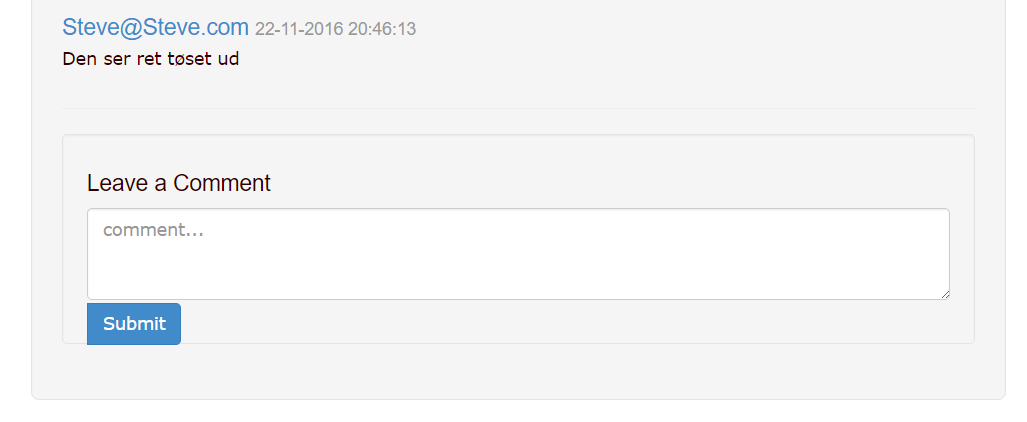
\includegraphics
 	[width=140mm]{../Dokumentation/figures/Kommentar.PNG}
 	\caption{Udseende af kommentarer}
 	\label{fig:Kommentar}
 \end{figure}
 
\noindent Viewet er lavet så det er intuitivt og nemt at overskue. Til viewet er der anvendt en bootstrap template \cite{kommentare}. Actionen til kommentering benytter Unit of Work som beskrives i \ref{sc:RepositoryPattern}, og virker efter principerne beskrevet i afsnit \ref{sc:GenerelControl}. Logikken til kommentarer er delvis genbrugt under ratings.